\section{Introduction}

\subsection{Présentation du projet}

Le COPEVUE a lancé un appel d'offre dans le cadre de la réalisation d'un système de monitoring de sites isolés. Il s'agit donc de concevoir en premier lieu une solution technique permettant de répondre au mieux aux exigences fonctionnelles et non fonctionnelles que le COPEVUE formule. De façon synthétique notre équipe va proposer une solution permettant de surveiller des sites naturels difficiles d'accès (souvent à cause des conditions environnementales) et peu peuplés. Dans ces sites isolés sont souvent regroupés des postes de travail et ces zones doivent pouvoir être surveillées en dépit de la distance qui les sépare du bureau de contrôle.

\subsection{Présentation du document}

Ce document permet de définir précisemment l'architecture applicative et technique de l'ensemble de notre solution, en rapport avec le dossier de Spécification Technique des Besoins. L'objectifs est d'apporté une réponse claire aux questions suivantes:

%Copier coller du doc de Regis
\begin{itemize}
	\item Quels sont les objets manipulés?
	\item Quelles sont les données manipulées?
	\item Analyse transformationnelle de ces données
	\item Description des stations locales et du système central
	\item Dimensionnement
	\item Analyse de la complexité
\end{itemize}

\section{Organisation générale du système}

\begin{figure}[hb]
  \centering
  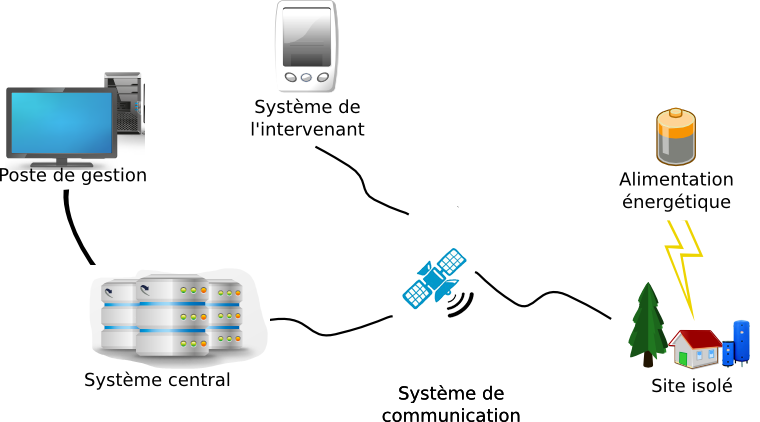
\includegraphics[width=15cm]{schema_architecture_generale_h4111_bis.png}
  \caption[Schéma de l'architecture globale]%
  {Schéma de l'architecture globale}
\end{figure}

\subsection{Système sur site isolé}

Chaque site isolé dispose d'un système complêt de monitoring du site, qui est décomposé de la manière suivante :

Les cuves à monitorer sont chacune équipées de capteurs relevant leur niveau de remplissage. Chaque capteur est géré par un composant connecté direcement dessus, que nous appelerons ici le ``système de gestion du capteur''. Ces systèmes fonctionneront ponctuellement, se réveillant de manière périodique pour effectuer des mesures à l'aide du capteur.

Le site est pourvu d'une ``station centrale'', principalement constituée d'un système embarqué à base d'OS Linux, qui va pouvoir communiquer avec les systèmes de capteurs vu précédement à l'aide d'une connexion sans-fil ZigBee. La station centrale aura elle aussi un fonctionnement ponctuel, se réveillant par tranches de 10 minutes toute les 6 heures (configuration par défaut), paramétrable bien évidement). Chaque fois qu'un système de gestion de capteur aura effectué une mesure, il essayera d'en communiquer le résultat à la base. En cas d'échec, il sera à même de conserver ces informations en vue d'une transmission ultérieur.\\
C'est un sous-système de la station centrale, le ``système de gestion du site'' qui sera responsable de la collecte des données auprès des capteurs, du maintient de la configuration de la station, mais aussi de la journalisation de données aussi bien logiques que physiques telles que les erreurs systèmes, la température extérieur, etc.

La station centrale dispose d'un autre sous-système, le ``système de transmission'', qui servira quant à lui à la communication avec le système central décrit plus loins. Cette transmission se fera de manière périodique, à une fréquence paramétrable, par satellite ou en utilisant le réseau GSM. Elle permettra d'envoyer dans un sens les relevés des capteurs, et dans l'autre l'envoi de nouveau paramètres de configuration à la station (et par extension, aux systèmes de gestion de capteurs).

\subsection{Système central}

Le ``système central'' est une application connectée à internet servant à centraliser les informations collectées sur l'ensemble des sites d'un territoire (voir même du monde). En voici le fonctionnement :

Les systèmes de transmission des sites isolés vont communiquer par internet avec le système central pour lui transmettre les derniers relevés des capteurs du site. Celui-ci va alors les stocker en base de données et vérifier si de nouvelles informations de configuration sont disponibles pour ce site. Si c'est le cas, celles-ci seront transmises en réponse.

En arrière plan, le système central va appliquer un ensemble de règles configurables pour vérifier si les nouvelles valeurs transmisent doivent déclencher des actions automatisées telles que des alertes ou des demandes d'intervention sur site.

Le système central va aussi présenter une interface de gestion au gestionnaires et clients du système, leur permettant de vérifier l'état et l'historique des mesures de chaque site, et la reconfiguration de ceux-ci. Cette interface doit aussi leur permettre de consulter d'éventuelles alertes, et de pouvoir y réagir en planifiant des interventions.

\subsection{Communication}

La communication entre la station et le central s’effectuera la plupart du temps en GSM. La plupart des sites isolés peuvent capter un signal, le GSM permet donc d’avoir une solution efficace, économe et peu cher. Dans le cas où aucune connexion GSM ne peut être faite, la base se connecte via satellite. La couverture des fournisseurs est quasi-totale, ce qui permet d’atteindre toutes les régions isolées. 

La communication entre les modules de capteurs et la base ce fait grâce au protocole ZigBee, qui permet de faire un réseau de plus de 60 000 appareil. Le ZigBee est très économes et le protocole est simple d’utilisation. Les cartes appliquant le ZigBee se paye a quelques dizaines d’euros. 

\section{Régles de pilotage du système}

\section{Architecture applicative}

\section{Architecture informatique et matérielle}

\subsection{Architecture matérielle}

\paragraph{Maintenance} Le technicien chargé de la maintenance du système est équipé d’un module capable de connecté à la station. Ce module doit être pourvu d’une prise USB pour relier l’appareil à la station. L’application de maintenance est utilisable sur un ordinateur  ou un matériel plus compact tel qu’un PDA ou un Smartphone. 

\paragraph{Capteur} Le module du capteur est équipé d’une carte contenant le capteur, le module de communication sans-fil et l’alimentation. Le système embarqué résiste aux conditions climatiques et a une très grande autonomie.

\paragraph{Base de la station} La base de la station est équipée du module de communication général  (GSM ou satellite selon la localisation du site), d’un module de communication ZigBee pour superviser le reste de la station. Cette base est capable d’enregistrer les informations les plus pertinentes avant de les retransmettre au central. La base est reliée à une source d’énergie qui l’alimente pendant de longue période. 

\subsection{Architecture informatique}

\paragraph{Module capteur} Le module capteur regroupe plusieurs parties logiciels. Le logiciel principal permet de vérifier le niveau de la batterie, de communiquer grâce au module ZigBee et de relever les valeurs du capteur. Pour cela un pilote est implémenté pour assurer une bonne intégration entre les éléments

\paragraph{Base de la station} La base est composé que d’un seul logiciel, qui a pour rôle de superviser la station. Elle doit ainsi relever les valeurs de tous les capteurs, les enregistrer et les retransmettre au central. Ce logiciel peut également reconfigurer différents éléments de la base telle que la période de réveil du système. Le protocole de communication implémenté est sécurisé, pour empêcher une interception des données ou une intrusion dans le système.

\section{Réflexions sur les données}

\subsection{Modèles de données du système}

, modèles de la base dedonnées intgrant les données de la prduction, volumétrie (évaluation de la base de données
pour une entreprise type en s’appuyant sur réflexion de l’annexe 1),

\subsection{Volume de données}

La première problématique qui se pose en regard du volume des données que nous allons devoir gérer est celle de la transmission de celles-ci depuis les sites jusqu'au serveur central. Les progrès récents en terme de transmission de données, autant par satellite que par réseau GSM, assurent un débit d'au moins 128kbps où que l'on se trouve dans le monde. Cela a pour conséquence de ne pas imposer de contrainte forte sur la taille des données que l'on souhaite transmettre. En effet, étant donné la nature de celles-ci, des valeurs de remplissage de cuves, au nombre d'une centaine par site au maximum, sur une période d'une journée (dans le cas où l'on souhaiterais une transmission quotidienne), on peut affirmer que chaque ``fichier'' envoyé par une station fera moins d'un MO. Les envoi étant effectués rapidement, c'est autant d'énergie qui sera économisée, augmentant ainsi la durée d'autonomie de chaque site.

L'autre aspect de la volumétrie des données est celle du stockage de l'historique des relevés de chaque site, et ce sur une longue période, pour être capable de les utiliser plus tard (e.g pour faire une comparaison des moyennes mensuelles d'une année à l'autre). Mais encore une fois, la nature des données concernée, et leur quantité, ne font pas de leur stockage une des principales difficultés de ce système, et un simple déploiement de serveurs SQL feront sans problème l'affaire.

\section{Gestion des problèmes et anomalies, sécurité}
Comme nous l'avons vu, la disponibilité du système est primordiale pour assurer une surveillance efficace des sites, c'est pourquoi il faut se prémunir contre les erreurs et surtout pouvoir gérer celles qui surviendraient pour éviter de paralyser tout le système. Notre architecture modulaire permet de limiter les risques, tous les éléments n'étant pas nécessaire au fontionnement de l'ensemble.
Dans l'architecture, la détection de problèmes matériels est également prévu, avec la possibilité de récupérer l'état des capteurs et autres composants, ce qui permet d'identifier l'origine des erreurs.
Le point névralgique de notre système est le dispositif de communication, son bon fonctionnement est primordial pour tous les autres composants qui gravitent autour. Il faut donc s'assurer de la qualité de service que l'opérateur choisi peut garantir. De notre côté, un soin tout particulier sera porté sur la résilience aux erreurs de ce module, pour ne pas pénaliser la bonne supervision des sites.
Un autre point important est le serveur central, qui matériellement ne présente que peu de risque, grâce au solution de Cloud Computing, par contre il faudra là aussi portée une grande attention à son comportement en cas d'erreur. Au niveau de la base de données, il est possible d'avoir des moyens de retours en arrière (rollback) en cas de corruption de celle-ci.


\section{Conclusion}

\section{Annexe 1 : Répresentation informatique des objets (messages…..)}

\section{Annexe 2 : Réflexion sur le réseau (principes qualité, pour la conception du réseau,
description du réseau (logiciel, couches…)…}

\section{Annexe 3 : Démarrage du système}
L'objectif est de voir comment le démarrage du système s'effectue.